\chapter{Protein fragments as search models in Molecular Replacement} \label{chap:ample_flib}
\clearpage

\section{Introduction}
\textit{Ab initio} structure prediction algorithms typically start with a coarse grained search of conformational space through the assembly of previously picked structural fragments. As such, the accuracy of structure prediction is heavily dependent on the similarity of fragments to the target fold for each position \cite{Gront2011-sv}. Thus, the necessary structural information for accurate structure prediction must be encoded in the fragment library for a given target sequence. This approach allows the modelling of new protein folds by considering them as assemblies of already known building blocks, such as super-secondary structure motifs \cite{Fernandez-Fuentes2010-ea}. Furthermore, fragments similar to those typically selected for \textit{ab initio} protein structure prediction were successfully used in other areas of Structural Biology including \gls{nmr} \cite{Delaglio2000-fx,Kontaxis2005-ea} and X-ray crystallography \cite{Jones1986-rd} studies to elucidate unknown protein folds. Despite their modest success, almost all attempts neglected target-specific information generally available to structural biologists obtainable through Bioinformatics software. This information includes the primary sequence of the target, torsion angle predictions, predicted solvent accessibility or coevolution information. In theory, all additional information should improve the generation of such fragment libraries by aiding the selection process or cross-validating the identified fragments.

Over the last decade, efforts have been made to improve the precision of structural fragment libraries used in \textit{ab initio} structure prediction \cite{Abbass2015-qk,Shen2013-wh,Li2008-xu,Kalev2011-sz,Bhattacharya2016-ix,Wang2017-ka,De_Oliveira2015-kb,De_Oliveira2018-za,Gront2011-sv}. Various different algorithms have been developed to generate static and dynamic fragment libraries. Static fragment libraries are those precomputed and generally consist of common super-secondary structure motifs. In comparison, dynamic fragment libraries consist of fragments of variable lengths acknowledging the fragment-dependent optimal length. Most commonly used in \textit{ab initio} structure prediction are dynamic algorithms, such as FLIB \cite{De_Oliveira2015-kb}, FLIB-COEVO \cite{De_Oliveira2018-za}, NNMAKE \cite{Gront2011-sv} or HHFRAG \cite{Kalev2011-sz}. Dynamic-library producing algorithms differ in their definition of ideal fragment lengths, the default number of fragments used per position and the way in which fragments are extracted. However, these algorithms typically share the same additional sequence-based information used to aid the selection of target fragments, which usually includes sequence similarity, three-state secondary structure prediction and torsion angle prediction.

Given that fragment libraries selected to perform \textit{ab initio} structure prediction can contain high quality fragments or super-secondary structure motifs, those fragments must sometimes be suitable as \gls{mr} search models. Correct identification of very similar fragments should allow for dynamic fragment selection to achieve \gls{mr} structure solution without the overhead of \textit{ab initio} structure prediction. Furthermore, dynamic algorithms could pick fragments of varying lengths, possibly matching coevolution data or other externally obtainable restraints to validate fragments prior to any \gls{mr} attempt. 

As such, the work in this chapter focused on exploring this idea using FLIB-COEVO \cite{De_Oliveira2018-za}, a dynamic fragment picking algorithm considering coevolution data to verify fragments during the picking procedure.

\section{Materials \& Methods}
\subsection{Target selection}
Four targets were manually selected for this study. The crystallographic data needed a resolution of around 1.5\AA\ with a single molecule in the asymmetric unit. The target chain length needed to be below 150 residues, and the fold of the protein structure to be either mixed \textalpha-\textbeta\ or all-\textbeta. A further target selection criterion was the availability of precise contact information for fragment selection.

The \gls{pdb} identifiers of the selected targets were: 1aba, 1lo7, 1u06, and 5nfc. The former two are described in \cref{table:appendix_dataset_original}. Target 1u06 is a more recently published structure of \textalpha-spectrin SH3 domain (\gls{pdb} ID: 1kjl in \cref{table:appendix_dataset_original}) with a resolution of 1.49\AA. Target 5nfc is a more recently published structure of Galectin-3 (\gls{pdb} ID: 1kjl in \cref{table:appendix_dataset_original}) with a resolution of 1.59\AA. This resulted in a dataset with similar attributes for each target: crystallographic data resolution of $~1.5$\AA\ with a single molecule in the asymmetric unit, and the target chain length of less than 150 residues. Each fold class, mixed \textalpha-\textbeta\ and all-\textbeta, contained two targets.

\subsection{Fragment picking using FLIB-COEVO}
FLIB-COEVO \cite{De_Oliveira2018-za} requires four inputs: the predicted secondary structure, predicted torsion angles, predicted or differently derived residue-residue contact pair data and a copy of the \gls{pdb}. The secondary structure for each target was predicted using PSIPRED v4.0 \cite{Jones1999-ed} with default parameters. The torsion angles were predicted using SPIDER v2 \cite{Heffernan2015-bt} with default parameters, and residue-residue contact pairs predicted with METAPSICOV v1.04 \cite{Jones2015-vq} with default parameters. HHBLITS v2.0.16 \cite{Remmert2011-kt} with \texttt{uniprot20} database v2016-02 was used by METAPSICOV to generate the \gls{msa} for contact prediction of each target sequence. BLASTP v2.2.31+ \cite{Altschul1990-og,Camacho2009-th} was used by PSIPRED with the \texttt{uniref90} database v2016-06. The local copy of the \gls{pdb} for fragment picking was downloaded on August 11, 2016.

Two modifications were made to the default FLIB-COEVO v1.01 (\url{https://github.com/sauloho/Flib-Coevo}, commit “\texttt{abade3b}”) protocol. The first focused on exclusion of fragments with $>90$\% helical content (assigned by DSSP \cite{Frishman1995-si}). If fragments with $>90$\% helical content were allowed and residues were predicted to be part of an \textalpha-helix, fragment libraries tended to be overpopulated for these positions with short helices. This would generate fragment libraries very similar to ideal-helix libraries, which was not the purpose of this work. The second modification was to allow fragments with \gls{rmsd} $>10.0$\AA\ to the reference structure to be considered. This modification to the FLIB-COEVO algorithm was implemented for development purposes by the authors to validate the performance of the algorithm. However, to allow for the automatic calculation of \gls{rmsd} value of each fragment without deliberately excluding less-similar fragments this constraint was lifted.

Two-hundred fragments were picked per target sequence position. Top-$L$ or $L/2$ contact pairs were selected from both METAPSICOV STAGE1 and STAGE2 predictions with a minimum sequence separation of either 6 or 12 residues. Helical fragments were either included or excluded. The fragment length ranged from either 6 or 12 (dependent on minimum sequence separation) to 63 residues. In all instances the \texttt{-coevo\_only} flag was set to exclude fragments with starting residues undefined by any contact pair in the set \footnote{The \texttt{-coevo\_only} flag was intended to select only fragments that satisfied at least one contact pair. This originally intended behaviour was not part of the source code throughout this study, and only detected post-analysis. The issue was reported to the developers and has since been fixed in the FLIB-COEVO source code (commit "\texttt{b3eb01d}").}. Overall, this generated 16 fragment libraries per target.

Each fragment library was then filtered to remove homologs of the target of interest to best replicate a blind study, in which this procedure may be relevant. BLASTP v2.2.31+ \cite{Altschul1990-og,Camacho2009-th} and HHPRED (HHBLITS v2.0.16 and HHSEARCH v2.0.16) \cite{Soding2005-sx} searches were conducted to identify homologous PDB entries. The BLASTP search was performed identically to \textcite{De_Oliveira2018-za} against the \texttt{pdbaa} v2016-10 database using an E-value cutoff of 0.05. The HHPRED search parameters were identical to the MPI-Toolkit \cite{Biegert2006-cb} web server version (\url{https://toolkit.tuebingen.mpg.de/}) and searches done against the \texttt{uniprot20} v2016-02 and \texttt{pdb70} v2016-09-14 databases. Fragments derived from PDB entries identified by BLASTP and HHPRED (probability score of $\geq20.0$) were excluded from the fragment libraries. This resulted in a much more rigorous homolog exclusion than similar \textit{ab initio} protein structure prediction studies would typically employ. However, in this study fragments were used directly as search models, and thus excluding even distantly related protein structures made it truly blind.

All per-target fragments were then binned by their peptide lengths. Subsequently, they were ranked by FLIB-COEVO scores and \gls{rmsd} values, and the best fragment from each length-dependent bin selected. Partially redundant fragments of the same template structure consisting of the same region with varying flanking residues were kept, if they were ranked top for each fragment length group. Finally, the coordinates of the fragment backbone atoms were extracted to create poly-alanine search models.

Note, the FLIB-COEVO score refers in this chapter to the predicted torsion angle score for a given fragment, which FLIB-COEVO uses in its default routine to rank fragments with lower scores being more favourable \cite{De_Oliveira2015-kb,De_Oliveira2018-za}. 

\subsection{Molecular Replacement in MRBUMP}
The previously extracted fragments were subjected to the \gls{mr} pipeline MRBUMP v0.9 shipped with CCP4 v7.0.28 \cite{Keegan2018-kn}. This uses PHASER \cite{McCoy2007-mp} for \gls{mr}, REFMAC5 \cite{Murshudov2011-ww} for refinement and SHELXE \cite{Thorn2013-le} for density modification and main-chain tracing. MRBUMP default parameters were used with exception of the PHASER \gls{rmsd} estimate. Each fragment was subjected to MRBUMP using PHASER \gls{rmsd} values of 0.1, 0.6 and 1.0\AA.

\subsection{Assessment of FLIB-COEVO fragments}
Fragment torsion angles --- predicted by SPIDER v2 \cite{Heffernan2015-bt} --- were assessed using the \gls{mae}, which evaluated the average absolute difference between the predicted and experimentally determined angles \cite{Heffernan2015-bt}. To account for the periodicity of an angle, the smaller value of the absolute difference $d_i$ and $360-d_i$ was used. The coverage of a fragment library was assessed by the proportion of residues present in at least one fragment in the library. The precision of a fragment library was defined by the fraction of \gls{tp} fragments. All fragments with an \gls{rmsd} of $<1.5$\AA\ were considered \gls{tp} else \gls{fp}. The equation used to calculated the precision score is \cref{eq:methods_contact_precision}. The \gls{rmsd} value, as calculated by FLIB-COEVO \cite{De_Oliveira2018-za}, was computed between the aligned residues of the corresponding crystal structure and the fragment. The number of satisfied contact pairs in each fragment was calculated by scoring the number of TP contact pairs by using a contact's residue indices according to the sequence alignment provided by FLIB-COEVO. \Gls{mr} success for each search model was solely assessed by SHELXE scores, whereby a \gls{cc} score of $\geq25.0$ combined with an \gls{acl} score of $\geq10.0$ was required.

\section{Results}
In this study, the main objective was to determine if peptide fragments derived from unrelated protein structures in the \gls{pdb} could be reliably identified and trialled in \gls{mr} to achieve structure solutions. The fragment picking algorithm FLIB-COEVO \cite{De_Oliveira2018-za} was used to pick fragments given its novel approach of validating selected fragments against a set of predicted residue-residue contacts.

\subsection{Precision of FLIB-COEVO input data}
The FLIB-COEVO algorithm requires two sets of input data --- the predicted secondary structure and per-residue torsion angles --- for each target sequence alongside an optional third source of information in form of coevolution data. The first part of the analysis in this study focused on these data given that the FLIB-COEVO fragment picking heavily relies on the individual features in the selection and scoring of each individual fragment \cite{De_Oliveira2018-za}. Poor data at this stage could lead to poor fragments that would be unsuitable for \gls{mr} trials given that high accuracy, i.e. a low \gls{rmsd} value between the search model and target, is required \cite{Scapin2013-yp}.

The secondary structure prediction highlighted high precision between each target's prediction and the DSSP-assigned \cite{Frishman1995-si} secondary structure of the target reference structure (\cref{fig:ample_flib_psipred}). The three targets with \gls{pdb} identifiers 1aba, 1lo7 and 1u06 had secondary structure predictions with a precision of $>89$\%. The fourth target, 5nfc, showed comparatively poor precision of 50.7\% over all residues in the PSIPRED prediction and the DSSP assignment using the reference crystal structure. However, 11 out of 13 secondary structure features were correctly predicted with deviations primarily found in the flanking residues of each secondary structure feature. 

\begin{figure}[H]
	\centering
	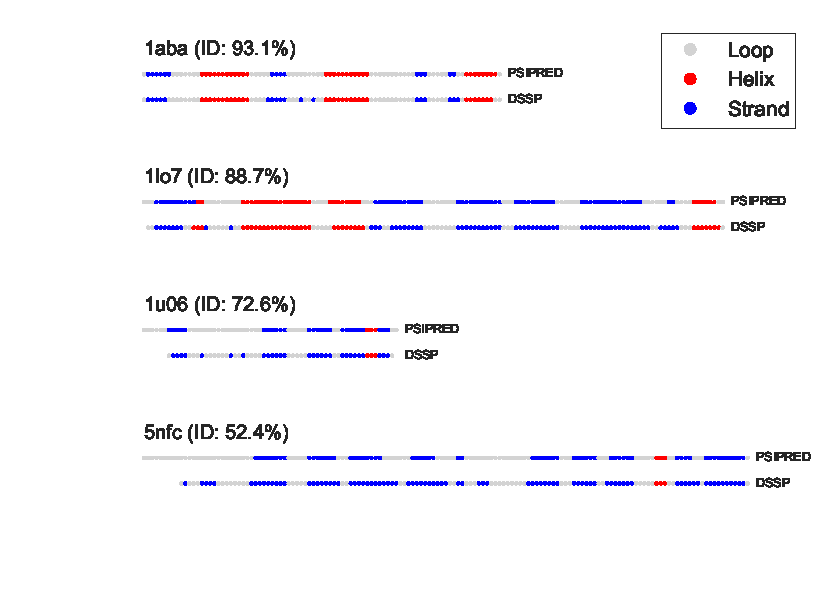
\includegraphics[width=\textwidth]{ample_flib_psipred.pdf}
	\caption[PSIPRED schema for FLIB-COEVO targets]{Schematic comparison of PSIPRED \cite{Jones1999-ed} secondary structure prediction and DSSP \cite{Frishman1995-si} assignment. Percentage identity is provided next to each identifier. The identity was computing using the Hamming distance over all positions present in the target sequence and reference structure.}
	\label{fig:ample_flib_psipred}
\end{figure}

The contact prediction data for METAPSICOV STAGE1 and STAGE2 predictions demonstrated the high precision achievable by this algorithm (\cref{table:ample_flib_contact_precision}). In this study, the top contact pairs at cutoffs $L$ and $L/2$ were provided to the FLIB-COEVO algorithm. All targets had precision scores for both sets of predictions at both cutoff levels of more at least 0.6 (\cref{table:ample_flib_contact_precision}). A comparison of the sets of predicted contact pairs showed that only every third (for $L/2$ contacts) or every other (for $L$ contacts) contact pair is shared between both METAPSICOV predictions highlighting the importance of trialling both when selecting FLIB-COEVO fragments (Jaccard index in \cref{table:ample_flib_contact_precision}).

\begin{table}[H]
  \centering
  \caption[Contact prediction summary for FLIB-COEVO targets]{Precision scores for METAPSICOV \cite{Jones2015-vq} STAGE1 and STAGE2 contact predictions. Jaccard index calculated for the same $L$-dependent selection of contact pairs between METAPSICOV STAGE1 and STAGE2 predictions.}
  \label{table:ample_flib_contact_precision}
  \begin{tabularx}{\textwidth}{X X X X X X X}
      \hline
	  \multirow{2}{*}{\textbf{Target}} & \multicolumn{3}{c}{\textbf{$L/2$ contact pairs}} & \multicolumn{3}{c}{\textbf{$L$ contact pairs}} 	\\ \cline{2-7}
	  							&  	Prec\textsubscript{STAGE1}	& 	Prec\textsubscript{STAGE2}	& 	Jaccard 	& 	Prec\textsubscript{STAGE1} 	& 	Prec\textsubscript{STAGE2} 	& 	Jaccard	\\
	  \hline
	  1aba						&	0.884	&	0.884	&	0.303	&	0.713	&	0.759	&	0.513		\\
	  1lo7						&	0.857	&	0.957	&	0.308	&	0.738	&	0.837	&	0.446		\\
	  1u06						&	0.839	&	0.806	&	0.378	&	0.710	&	0.787	&	0.459		\\
	  5nfc						&	0.822	&	0.836	&	0.327	&	0.619	&	0.762	&	0.434		\\ 
	  \hline
  \end{tabularx}
\end{table}

Given the two METAPSICOV contact prediction files, both showed localised clusters of contact pairs characteristic for secondary structure features (\cref{fig:ample_flib_cmaps}). These clusters were more populated with contact pairs in METAPSICOV STAGE2 predictions. This behaviour is to-be-expected given that the second stage in METAPSICOV screens the first to remove singleton contact pairs whilst enriching the already existing clusters \cite{Jones2015-vq}. Besides the visual analysis, a cluster determination study on each of those contact maps further confirmed a higher singleton frequency in METAPSICOV STAGE1 predictions. The latter contained on average 9\% more singleton contact pairs, and thus a higher degree of noise.

\begin{figure}[H]
	\centering
	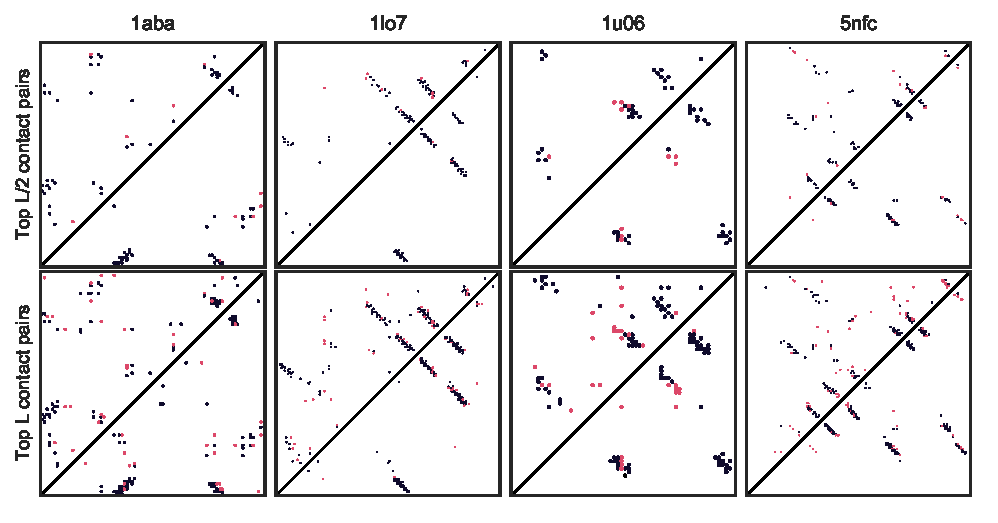
\includegraphics[width=\textwidth]{ample_flib_cmaps.pdf}
        \caption[Contact map comparison for FLIB-COEVO targets]{Comparison of $L/2$ and $L$ correctly and incorrectly predicted contact pairs for four FLIB-COEVO targets. Contacts were predicted using METAPSICOV \cite{Jones2015-vq} STAGE1 (top left) and STAGE2 (bottom right). \Gls{tp} and \gls{fp} contact pairs were identified using an 8\AA\ cutoff between C\textalpha\ (C\textbeta\ in case of Gly) atoms of a reference crystal structure. PSIPRED \cite{Jones1999-ed} secondary structure prediction provided along the diagonal.}
	\label{fig:ample_flib_cmaps}
\end{figure}

An analysis of the \gls{mae} of torsion angles between the SPIDER2 \cite{Heffernan2015-bt} prediction and a corresponding reference crystal structure highlighted accurate predictions for three of four targets (\cref{fig:ample_flib_spider2}). The largest \gls{mae}\textsubscript{\textphi} across the four target sequences was $24.347^{\circ}$, and the largest \gls{mae}\textsubscript{\textpsi} was $45.459^{\circ}$ (\gls{mae} values for \gls{pdb} entry 1u06). The smallest \gls{mae}\textsubscript{\textphi} was $13.822^{\circ}$ (\gls{pdb} ID: 1aba) and smallest \gls{mae}\textsubscript{\textpsi} was $17.273^{\circ}$ (\gls{pdb} ID: 1lo7). Segments in sequence space with regular secondary structure, as predicted by PSIPRED \cite{Jones1999-ed}, resulted primarily in low \gls{mae} values of torsion angles. In contrast, unstructured regions highlighted much larger \gls{mae} values indicating the difficulty of predicting these regions. Noticeably, the \gls{mae}\textsubscript{\textpsi} appeared to be much larger in those regions than the \gls{mae}\textsubscript{\textphi} for the same residue.

In summary, all target sequences had FLIB-COEVO input data of good quality, which should allow FLIB-COEVO to select fragments of suitable accuracy for \gls{mr}.

\begin{figure}[H]
	\centering
	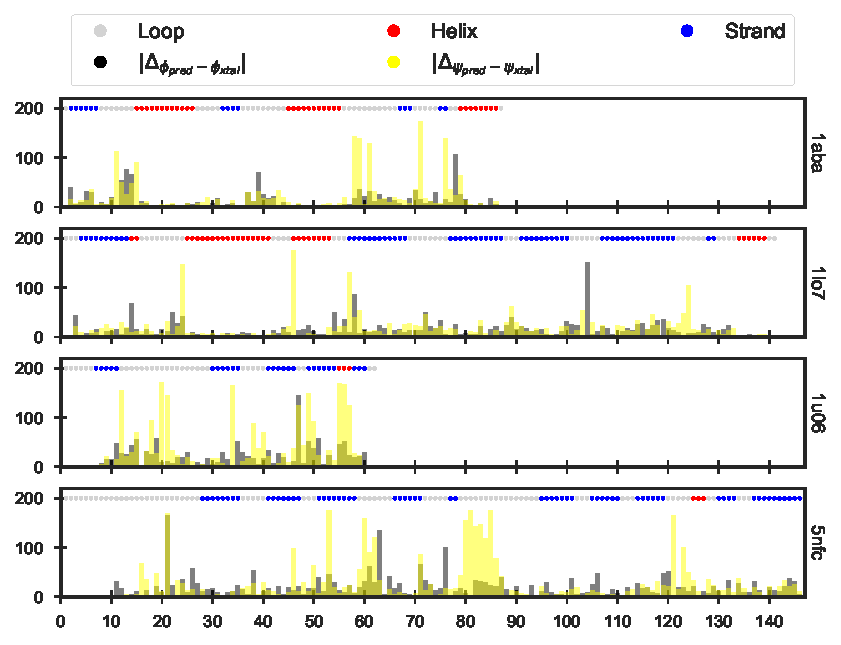
\includegraphics[width=\textwidth]{ample_flib_spider2.pdf}
	\caption[SPIDER2 torsion angle prediction analysis of FLIB-COEVO targets]{Comparison of \gls{mae} of torsion angles predicted by SPIDER2 \cite{Heffernan2015-bt} and extracted from a corresponding \gls{pdb} structure. PSIPRED \cite{Jones1999-ed} secondary structure prediction provided alongside the \gls{mae} values.}
	\label{fig:ample_flib_spider2}
\end{figure}

\subsection{FLIB-COEVO fragment picking}
Sixteen FLIB-COEVO fragment libraries were created for each protein target in this study. Each fragment library consisted of one combination of one of two contact prediction files and altering input parameters.

Across all four targets, the FLIB-COEVO algorithm selected a total of 8,535,458 fragments (\cref{table:ample_flib_frag_summary}). The fragment libraries showed similar statistics across the four protein targets despite the diversity in fold and chain lengths. The mean FLIB-COEVO score was ~3,200 score units with a mean \gls{rmsd} of 9.00\AA. Fragments for the alpha-spectrin SH3 domain (\gls{pdb} ID: 1u06) scored the lowest mean FLIB-COEVO score with 3,034 units; however, the same target scored the worst by mean \gls{rmsd} with an average of 9.47\AA. In contrast, fragments picked for the sequence of the bacteriophage T4 glutaredoxin (\gls{pdb} ID: 1aba) achieved the best mean \gls{rmsd} of 7.85\AA\ given the second highest mean FLIB-COEVO score of 3,217 units (\cref{table:ample_flib_frag_summary}).

\begin{table}[H]
  \centering
  \scriptsize
  \caption[FLIB-COEVO fragment characterics across four protein targets]{Summary of fragment statistics for FLIB-COEVO libraries selected for four protein targets. Count\textsubscript{H} corresponds to the count of fragments extracted from homologs.}
  \label{table:ample_flib_frag_summary}
  \begin{tabularx}{\textwidth}{X X X X X X X X X}
      \hline
      \multirow{2}{*}{\textbf{Target}} & \multirow{2}{*}{\textbf{Count}} & \multirow{2}{*}{\textbf{Count\textsubscript{H}}} & \multicolumn{3}{c}{\textbf{FLIB-COEVO score}} & \multicolumn{3}{c}{\textbf{\gls{rmsd}}} \\ \cline{4-9}
      		&			&			& Median 	& Mean 		& Std Dev 	& Median 	& Mean 	& Std Dev \\
      \hline
      1aba	& 2,091,321	& 45,133		& 3,061	& 3,217	& 1,405	& 7.70	& 7.85	& 3.81	\\
	  1lo7	& 2,497,813	& 23,396		& 3,187	& 3,371	& 1,497	& 9.00	& 9.43	& 4.61	\\
      1u06	& 1,133,517	& 60,159		& 2,901	& 3,034	& 1,306	& 9.51	& 9.47	& 3.94	\\
      5nfc	& 2,812,807	& 48,828		& 2,982	& 3,127	& 1,316	& 8.89	& 9.16	& 4.18	\\
      \hline
      Total	& 8,535,458	& 177,516		& 3,049	& 3,208	& 1,397	& 8.68	& 8.96	& 4.25	\\
      \hline
  \end{tabularx}
\end{table}

\begin{figure}[H]
	\centering
	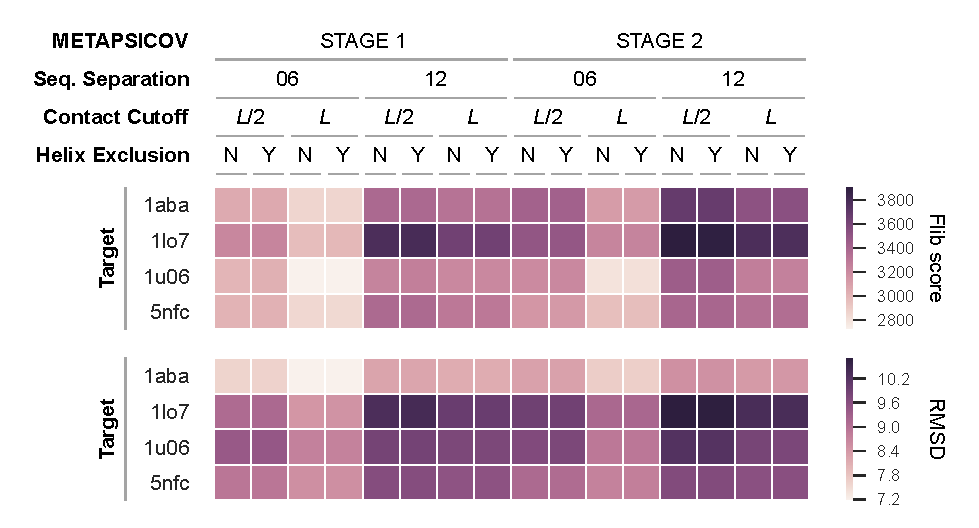
\includegraphics[width=\textwidth]{ample_flib_flibcond.pdf}
	\caption[FLIB-COEVO fragment library comparison]{FLIB-COEVO fragment library comparison for four targets highlighting the differences in mean FLIB-COEVO score and \gls{rmsd} by starting with different subsets of contact predictions. $L$ refers to the number of residues per target sequence. $Y$ refers to idealised \textalpha-helical fragment exclusion during fragment picking; $N$ refers to treating those fragments like all others.}
	\label{fig:ample_flib_flibcond}
\end{figure}

A split of the per-target fragment libraries by input options highlighted the better fragment library quality under certain conditions with regards to the mean FLIB-COEVO score and \gls{rmsd} (\cref{fig:ample_flib_flibcond}). In particular, top-$L$ (6 residues sequence separation) METAPSICOV STAGE1 contact predictions yielded the lowest for both metrics across all targets. A comparison of the sequence separation, i.e. using all contact pairs or medium- and long-range ones only, strongly suggested much lower and thus more favourable scores for using short-, medium- and long-range contact pairs. A very similar difference was noticeable for METAPSICOV STAGE2 contact predictions (\cref{fig:ample_flib_flibcond}). 

In this study, predicted contact information was used to further guide fragments selection. The FLIB-COEVO algorithm only selected fragment for positions of the target sequence with at least one contact pair. Given this scenario, an analysis of the coverage of the target sequence with respect to each picking strategy further demonstrated the benefits of starting with METAPSICOV STAGE1, i.e. noisier contact predictions (\cref{fig:ample_flib_fragtps}). Coverage was more evenly spread across the target sequences compared to missing regions especially for target 4-hydroxybenzoyl CoA thioesterase (\gls{pdb} ID: 1lo7) when starting with METAPSICOV STAGE2 predictions. Noticeably, none of the picking strategies yielded any fragments for the C-termini of \textalpha-spectrin SH3 domain (\gls{pdb} ID: 1u06) and galectin-3 CRD (\gls{pdb} ID: 5nfc) (\cref{fig:ample_flib_fragtps}). Furthermore, an analysis of the precision of fragments in each library strongly supported the benefits of starting with top-$L$ (6 residues sequence separation) METAPSICOV STAGE1 contact pairs. Across all four targets, the coverage of correct fragments (classed by \gls{rmsd} $<1.5$\AA\ to the reference structure) was highest for this condition. This is of particular importance for \textalpha-spectrin SH3 domain (\gls{pdb} ID: 1u06) and galectin-3 CRD (\gls{pdb} ID: 5nfc), for which most strategies picked very few to no correct fragments. Excluding idealised \textalpha-helical fragments did not affect the quality of the FLIB-COEVO libraries greatly. A consideration of differences in mean FLIB-COEVO and \gls{rmsd} scores showed differences of 25.68 and 0.06 between comparable libraries, i.e. with and without idealised \textalpha-helical fragments.

Given that FLIB-COEVO used coevolution data to help select fragments, it was little surprise that higher degrees of \gls{tp} fragments colocalise with high-density contact pair regions along the target sequence (\cref{fig:ample_flib_fragtps}). This characteristic explained less \gls{tp} fragments in top-$L/2$ fragment libraries because less contacts (compared to top-$L$) were available during fragment selection. The resulting selection was purely based on the FLIB-COEVO score which might not yield high-accuracy fragments (\gls{rmsd} $<1$\AA) as frequently. Therefore, the co-localisation of \gls{tp} FLIB-COEVO fragments and regions of high-density contact predictions highlighted the importance of adding this additional source of information to pick fragments. 

\begin{figure}[H]
	\centering
	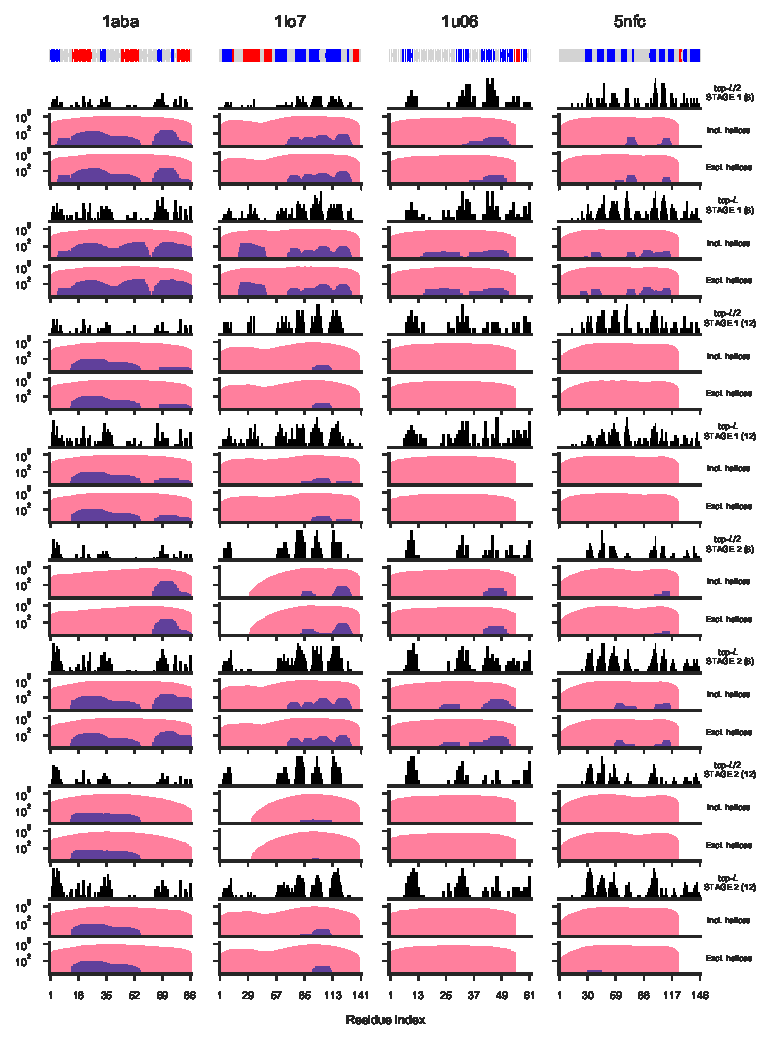
\includegraphics[width=\textwidth]{ample_flib_fragtps.pdf}
	\caption[Coverage and precision of Flib fragment libraries]{Summary of the coverage and precision of FLIB-COEVO fragment libraries according to their target sequence. The coverage of all fragments with respect to their target-aligned sequence register are shown in red bars, and fragments with \gls{rmsd} $<1.5$\AA\ to the reference structure in blue. The predicted secondary structure of each target sequence is given at the top: \textalpha-helices (red), \textbeta-strands (blue), and loops (grey). Contact prediction information is illustrated using black bars. The fragment frequency is shown using a log-scale.}
	\label{fig:ample_flib_fragtps}
\end{figure}

\subsection{FLIB-COEVO fragment selection for Molecular Replacement}
One of the most challenging and important aspects of bypassing \textit{ab initio} protein structure prediction to use the picked fragments directly as \gls{mr} search models is the accurate identification of fragments with the highest similarity between fragment and target structure.

\begin{figure}[H]
	\centering
	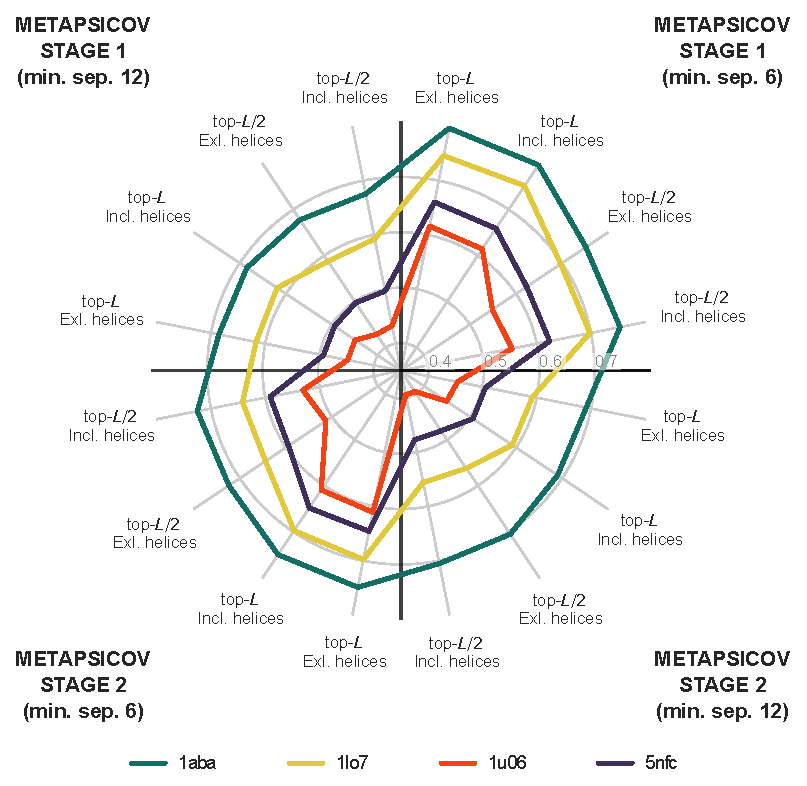
\includegraphics[width=\textwidth]{ample_flib_flibspearman.pdf}
        \caption[Correlation coefficient analysis of FLIB-COEVO fragments]{Spearman rank-order correlation coefficient analysis of FLIB-COEVO fragments' FLIB-COEVO score and \gls{rmsd} value given the 16 unique fragment picking strategies across four targets. P-values of all Spearman correlations are $<0.001$ and not shown for simplicity of the plot.}
	\label{fig:ample_flib_flibspearman}
\end{figure}

A fragment's FLIB-COEVO score --- its cumulative absolute error of predicted torsion angles --- has the highest correlation with the \gls{rmsd} of a fragment compared to all other scores used in the FLIB-COEVO protocol \cite{De_Oliveira2018-za}. To validate this finding, all non-homologous fragments in this study were tested for a correlation between their FLIB-COEVO scores and \gls{rmsd} values. The Spearman's rank-order correlation coefficient analysis confirmed the correlation between a fragment's FLIB-COEVO and \gls{rmsd} scores (\cref{fig:ample_flib_flibspearman}). However, the strength of the correlation varied greatly between different fragment libraries and targets. The optimal fragment picking strategy --- top-$L$ (6 residues sequence separation) METAPSICOV STAGE1 --- resulted in the strongest correlations across all targets. The same contact pair selection with METAPSICOV STAGE2 predictions results in the second strongest correlation. Noticeably, the bacteriophage T4 glutaredoxin (\gls{pdb} ID: 1aba) fragment libraries showed stronger positive correlations than the remaining targets. The fragments selected for \textalpha-spectrin SH3 domain (\gls{pdb} ID: 1u06) showed the overall weakest correlations. It is worth noting that the two targets (\gls{pdb} IDs: 1aba \& 1lo7) were classed as mixed \textalpha-\textbeta\ targets, and thus the strength of this correlation might be fold-dependent.

Further inspection of the fragments and the relationship between each fragment's FLIB-COEVO score and \gls{rmsd} value revealed a small subset of outliers in each fragment library. These fragments (hereafter referred to as outlier fragments) were sparse in each library with an overall mean count of less than 0.2\%. An analysis for unique characteristics of these outliers, which would allow for their exclusion, revealed no unique feature. These fragments contained all secondary structure types, spanned across all target sequences and ranged over all peptide lengths. Furthermore, they occurred in all fragment libraries, irrelevant of their original picking strategy. The only characteristic setting these outlier fragments apart from the remaining set was a \gls{rmsd} value of $>30$\AA. Nevertheless, it appeared that these outlier fragments with unusually high \gls{rmsd} values were never included in the final fragment search model set, given that their overall FLIB-COEVO\textsubscript{min} score was 796 units (one order of magnitude more than the overall minimum for the remaining fragments).

An analysis of the fragment metrics in the final \gls{mr} set (6,547 fragments) further supported the positively linear relationship between a fragment's FLIB-COEVO score and \gls{rmsd} (\cref{fig:ample_flib_finalrelat}a). However, the best FLIB-COEVO fragments by \gls{rmsd} showed much less spread compared to the best fragments by FLIB-COEVO score (\cref{fig:ample_flib_finalrelat}b). Furthermore, the size of the fragments also positively correlated with the FLIB-COEVO ($\rho_{Spearman}=0.860$, $p<0.001$) and \gls{rmsd} ($\rho_{Spearman}=0.697$, $p<0.001$) values. Longer fragments with higher dissimilarity with respect to the target showed higher FLIB-COEVO scores and \gls{rmsd} values (\cref{fig:ample_flib_finalrelat}a). 

\begin{figure}[H]
	\centering
	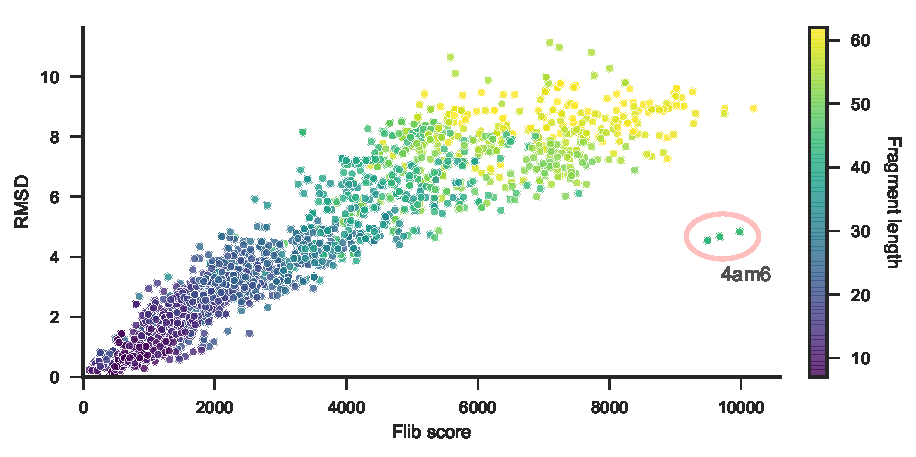
\includegraphics[width=\textwidth]{ample_flib_finalrelat.pdf}
        \caption[Correlation analysis for FLIB-COEVO MR fragments]{Scatter plot highlighting the positive correlation between fragment FLIB-COEVO scores and \gls{rmsd} values. The plot contains all fragments independent of target or picking strategy. \textbf{a.} The colour of each scatter point illustrates the fragment length. All extreme outlier fragments are highlighted with their \gls{pdb} identifiers as labels. \textbf{b.} The colour codes indicate the sorting strategy to select the top FLIB-COEVO fragments for each fragment peptide length bin.}
	\label{fig:ample_flib_finalrelat}
\end{figure}

Notably, a cluster of large fragments with some of the highest FLIB-COEVO scores in the set showed a reasonable similarity to their target structure (\cref{fig:ample_flib_finalrelat}a). All fragments in this cluster were picked for the bacteriophage T4 glutaredoxin sequence (\gls{pdb} ID: 1aba) and extracted from the same region of the crystal structure of the actin-related protein ARP8 (\gls{pdb} ID: 4am6). In comparison, some smaller fragments with peptide lengths less than 50 residues and lower FLIB-COEVO scores of less than 3000 showed the highest \gls{rmsd} values in the final set.

One further unique aspect of this study compared to other fragment-\gls{mr} approaches was the use of predicted residue-residue contact information to select fragments during picking, only selecting fragments for target-sequence residues with at least one contact pair in the predicted set (Saulo de Oliveira, personal communication). In the final set, 39\% of all fragments satisfied at least one, 26\% at least two and 20\% at least three contact pairs. Across the four targets, 50\% of all fragments selected for 4-hydroxybenzoyl CoA thioesterase (\gls{pdb} ID: 1lo7) satisfied at least one predicted contact pair (\cref{fig:ample_flib_consatis}). In comparison, 28\% of fragments selected for the \textalpha-spectrin SH3 domain (\gls{pdb} ID: 1u06) satisfied at least one contact pair.

\begin{figure}[H]
	\centering
	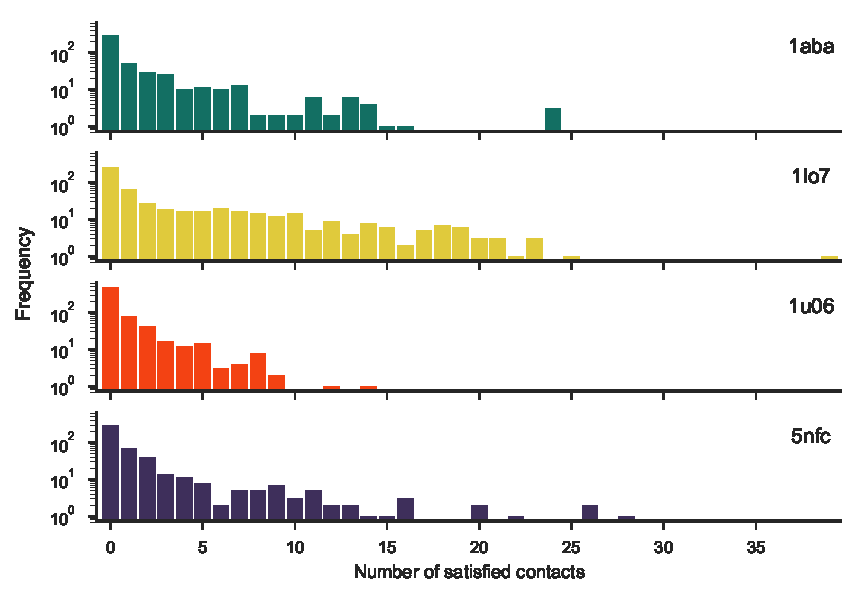
\includegraphics[width=\textwidth]{ample_flib_consatis.pdf}
	\caption[Distribution of contact precision for FLIB-COEVO fragments]{Distribution of contact precision for FLIB-COEVO fragments selected as \gls{mr} search models separated on a per-target basis.}
	\label{fig:ample_flib_consatis}
\end{figure}

Thus, the final set of FLIB-COEVO fragment \gls{mr} search models spanned a wide range of peptide lengths, \gls{rmsd} values, predicted contact satisfaction scores, and generally secondary structure make-up. To illustrate the latter, a random selection of sample fragments is illustrated in \cref{fig:ample_flib_search_models}. Importantly, not a single super-secondary structure motif dominated the set, increasing the sampling diversity to be undertaken during \gls{mr}.

\begin{figure}[H]
	\centering
	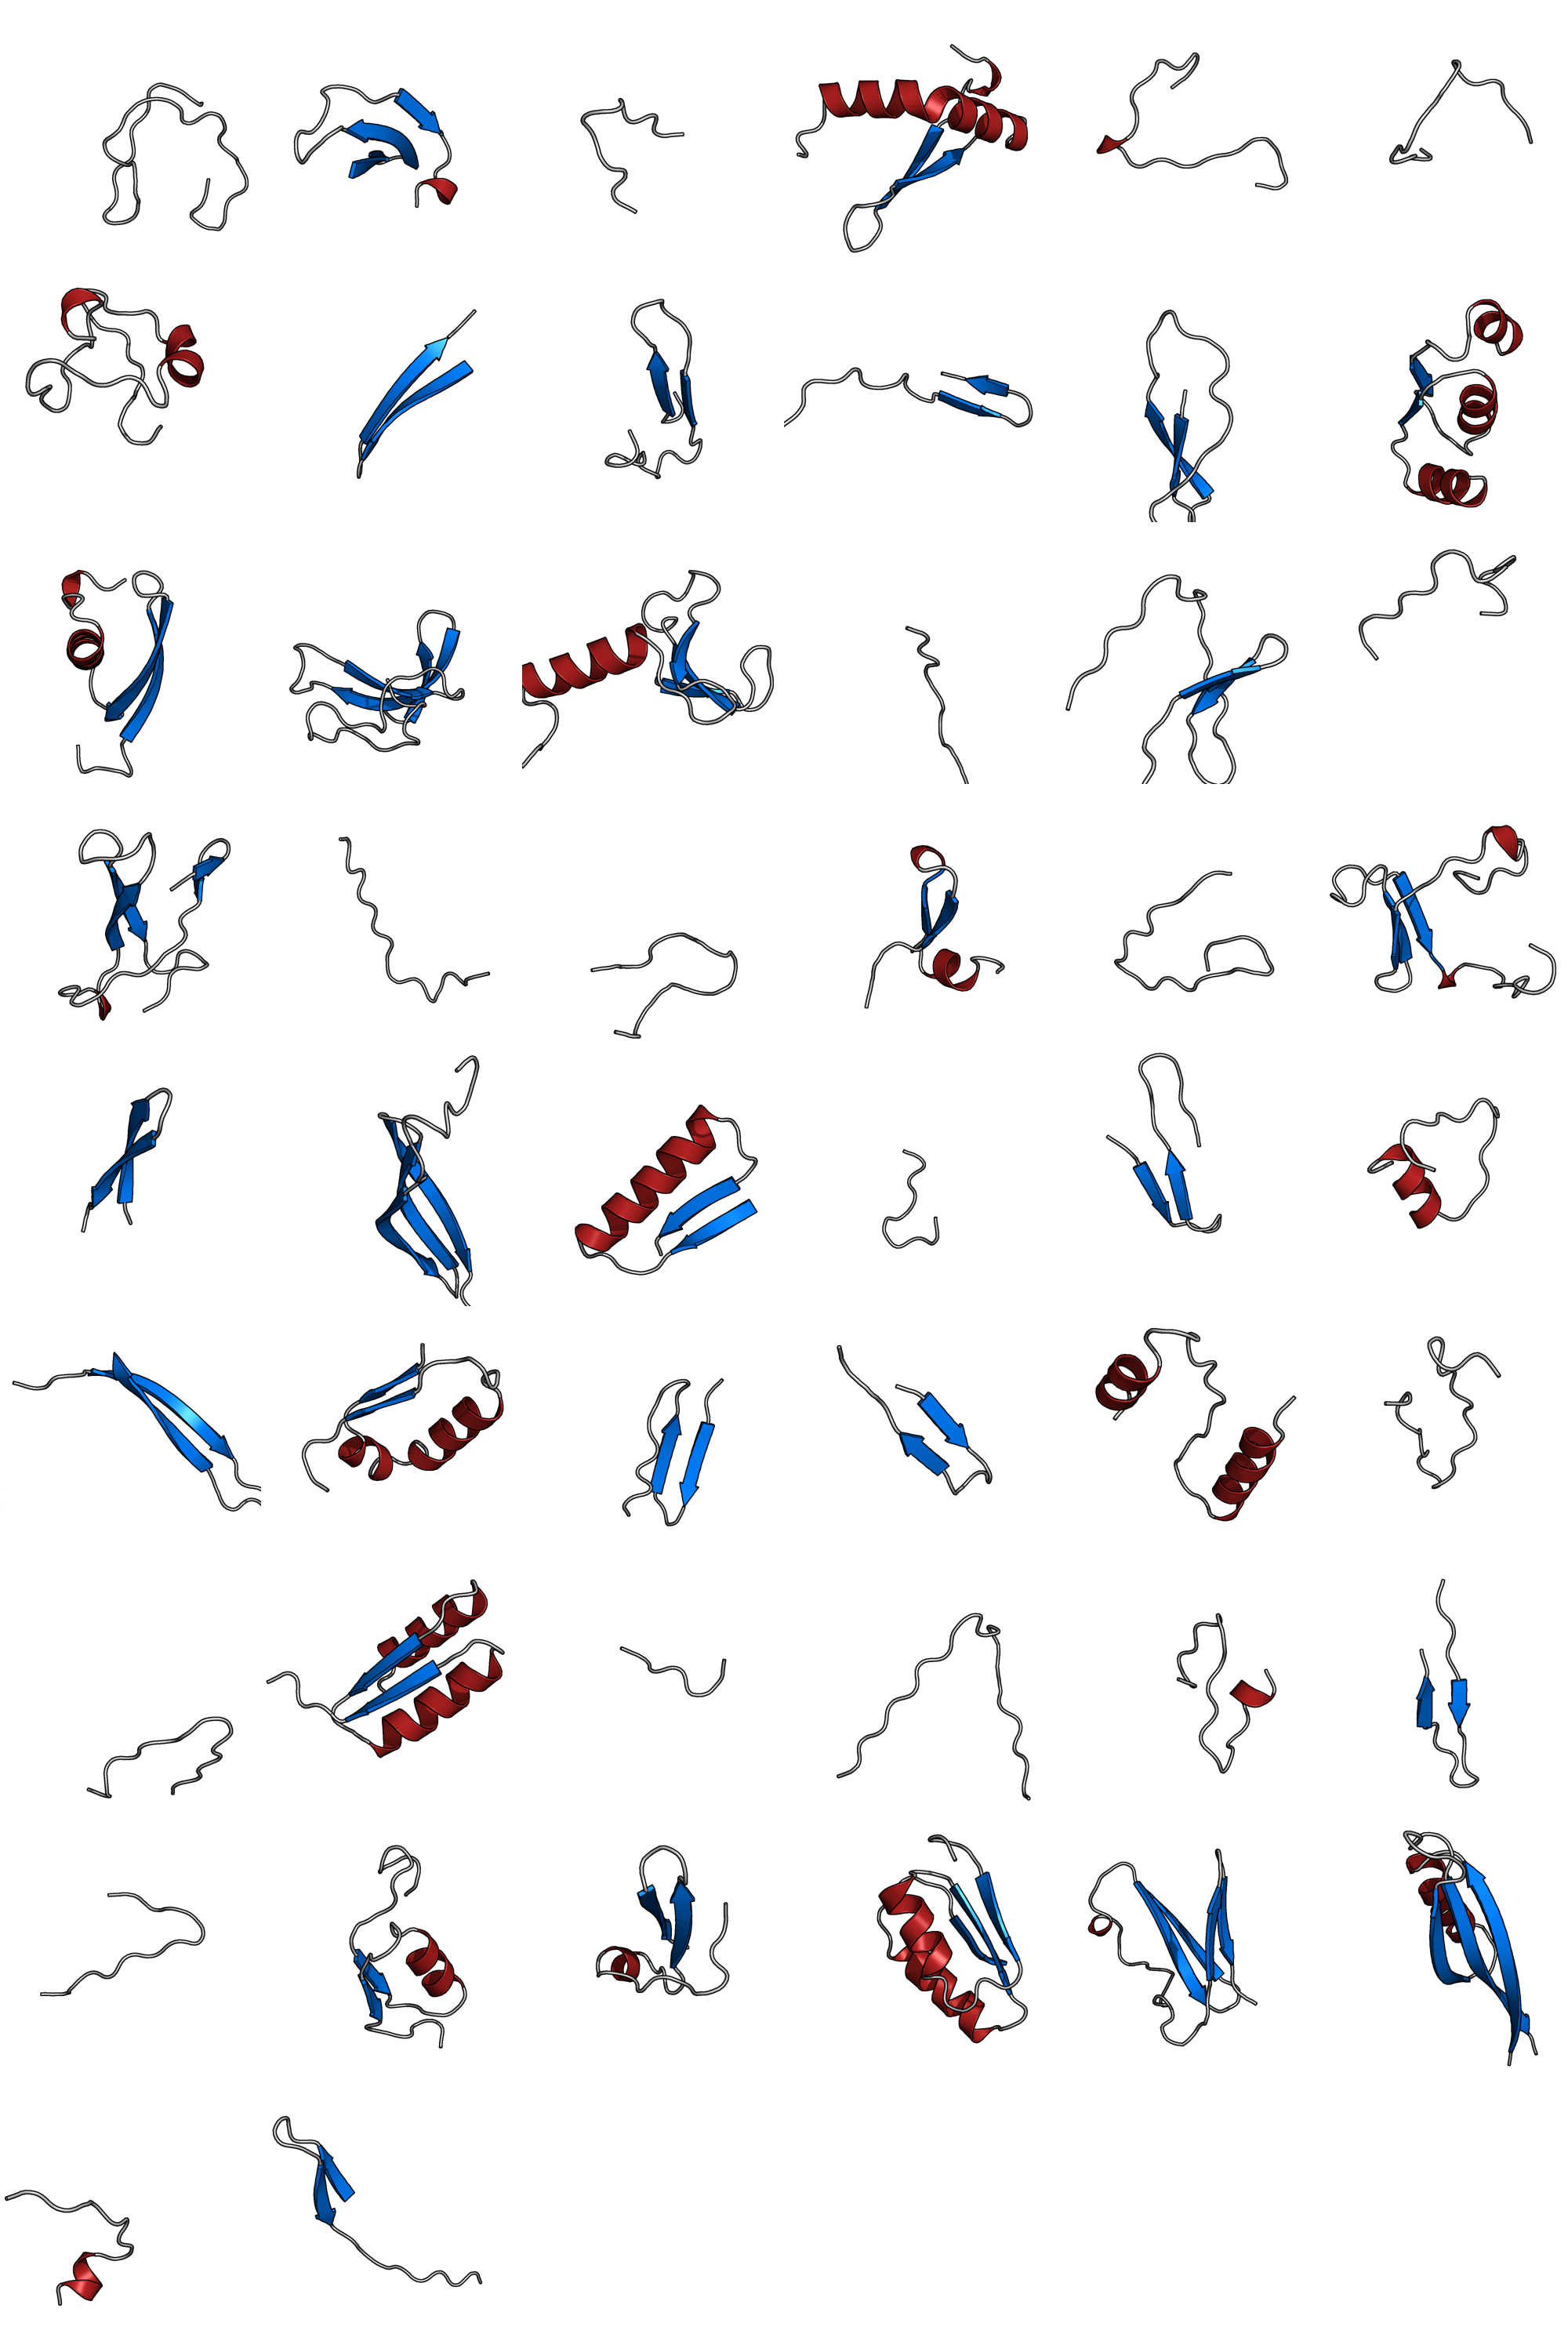
\includegraphics[width=\textwidth]{ample_flib_search_models2.png}
	\caption[Fragment search models derived from FLIB-COEVO]{Non-redundant sample of FLIB-COEVO fragment search models selected for four different protein targets. Secondary structure defined by and visualisation done in PyMOL \cite{Delano2002-hm}. Unpaired \textbeta-strands rendered using the loop style.}
	\label{fig:ample_flib_search_models}
\end{figure}

\subsection{Molecular Replacement using FLIB-COEVO fragments}
FLIB-COEVO fragments picked for four target sequences using a variety of FLIB-COEVO input options generated more than 6,500 fragments, which were subjected to the \gls{mr} pipeline MRBUMP with their corresponding target experimental data. Given that each fragment was trialled with three different PHASER \gls{rmsd} values, a total of 19,716 \gls{mr} attempts were made across four target structures. Out of nearly 20,000 \gls{mr} attempts, 299 led to the successful structure solution of two targets, namely the T4 glutaredoxin (\gls{pdb} ID: 1aba) and \textalpha-spectrin SH3 domain (\gls{pdb} ID: 1u06) (\cref{fig:ample_flib_mrsummary}).

\begin{figure}[H]
	\centering
	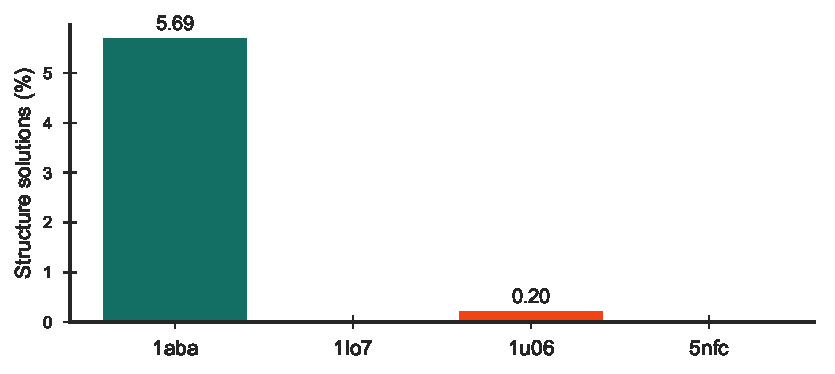
\includegraphics[width=\textwidth]{ample_flib_mrsummary.pdf}
	\caption[MR structure solutions by FLIB-COEVO target]{Distribution of structure solutions by FLIB-COEVO target. All \gls{mr} attempts total to 19,716, out of which 299 are structure solutions. Values above each bar indicates percentage search models successful out of the corresponding set.}
	\label{fig:ample_flib_mrsummary}
\end{figure}

The total of 299 \gls{mr} structure solutions were achieved by 70 sequence-unique fragments. Sixty-nine of those fragments were picked from 60 unique structures for the T4 glutaredoxin (\gls{pdb} ID: 1aba) leading to 97\% of all structure solutions. In comparison, a single fragment, selected from three different fragment libraries, led to nine structure solutions of the \textalpha-spectrin SH3 domain (\gls{pdb} ID: 1u06). The largest FLIB-COEVO fragment leading to a structure solution contained 37 residues and the smallest ten.

A division of FLIB-COEVO-fragment search models by their respective origin libraries provided strong evidence that METAPSICOV STAGE1 contact predictions allows for the selection of the most accurate fragments (\cref{fig:ample_flib_flibcond}), which directly translated into the structure solution count (\cref{fig:ample_flib_flibcondmr}). Furthermore, this division also highlighted and supported the quality of fragment libraries picked with top-$L$ (6 residues sequence separation) METAPSICOV STAGE1 predictions. Trialling the optimal fragment picking strategy with and without helical fragments ($>90$\% \textalpha-helical content assigned using DSSP) resulted in the library without outperforming the other (\cref{fig:ample_flib_flibcondmr}, 3\textsuperscript{rd} and 4\textsuperscript{th} bars). 

\begin{figure}[H]
	\centering
	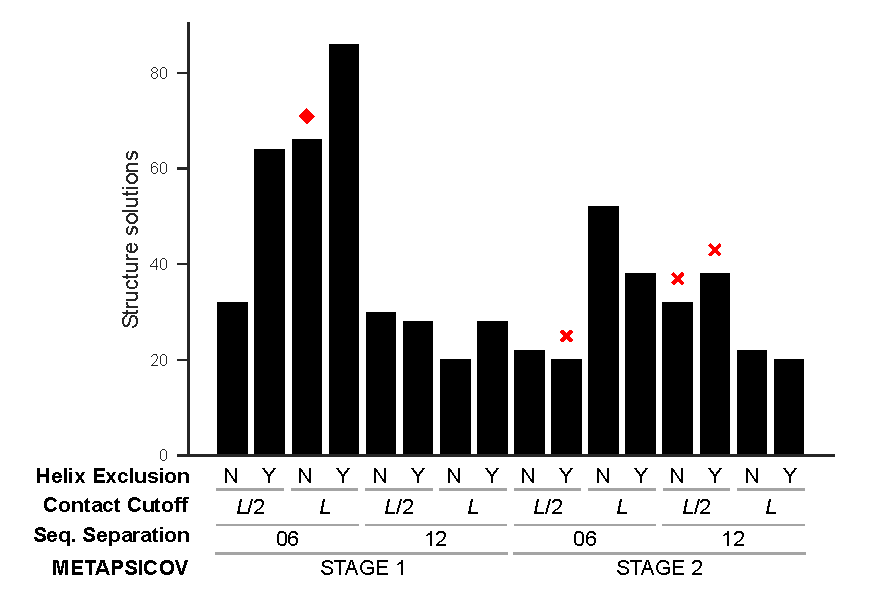
\includegraphics[width=\textwidth]{ample_flib_flibcondmr.pdf}
	\caption[MR structure solutions by FLIB-COEVO library]{Distribution of structure solutions by FLIB-COEVO library configuration. The optimal fragment picking strategy, as assessed by FLIB-COEVO values, is highlighted with a red diamond to illustrate that the method that picks the best fragments is close to, but not the absolute best for ultimate structure solution. Fragment picking strategies leading to solutions of \textalpha-spectrin SH3 domain (\gls{pdb} ID: 1u06) are highlighted with red crosses.}
	\label{fig:ample_flib_flibcondmr}
\end{figure}

An analysis of the binned results by fragment-ranking or PHASER \gls{rmsd} value confirmed the expected outcome: the top fragments selected by fragment \gls{rmsd} score result in more structure solutions than their FLIB-COEVO score counterparts (\cref{fig:ample_flib_mrbyconfig}). To reiterate, all FLIB-COEVO fragments were grouped by their peptide length, and the top fragment in each group selected when sorted by either FLIB-COEVO or \gls{rmsd} values. When separating the total number of structure solutions by the score that made each fragment the best in its original library, it became clear that two-thirds of solutions were achieved with fragments scoring best by \gls{rmsd}. However, the structure of \textalpha-spectrin SH3 domain (\gls{pdb} ID: 1u06) was only solved with fragments that scored best in their FLIB-COEVO fragment libraries by FLIB-COEVO score. A further subdivision of successful fragments, sorted either by FLIB-COEVO scores or \gls{rmsd} values, highlighted that a larger proportion of successful \gls{rmsd}-sorted fragments satisfied at least one predicted contact (FLIB-COEVO-sorted: 7\%; \gls{rmsd}-sorted: 13\%). A separation of attempts by PHASER \gls{rmsd} value suggested a value of 0.1 to be the most favourable.

\begin{figure}[H]
	\centering
	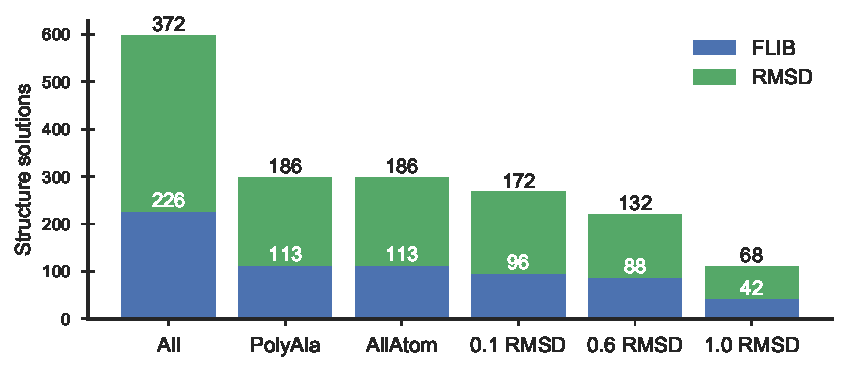
\includegraphics[width=\textwidth]{ample_flib_mrbyconfig.pdf}
	\caption[MR structure solutions by input parameters]{Distribution of structure solutions by fragment and MRBUMP configuration. The structure solution count is provided above each bar.}
	\label{fig:ample_flib_mrbyconfig}
\end{figure}

\begin{figure}[H]
	\centering
	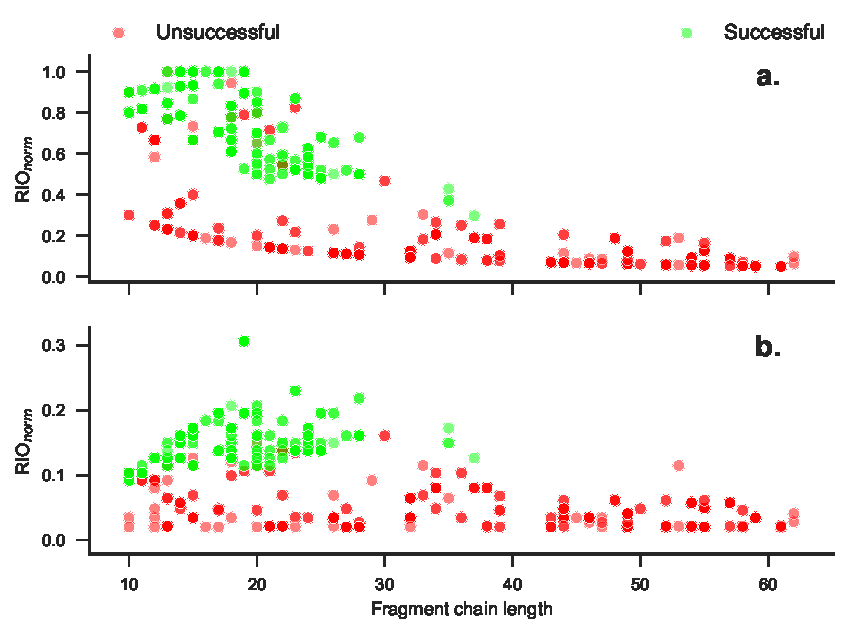
\includegraphics[width=\textwidth]{ample_flib_mrrionorm.pdf}
	\caption[Relationship between fragment chain length and RIO scores]{Dependence of normalised \acrlong{rio} (RIO\textsubscript{norm}) score on the fragment chain length. The two plots show  \gls{rio} scores normalised by the chain lengths of (a) the fragment and (b) the target. Colour coding indicates if the FLIB-COEVO-fragment search model resulted in a structure solution. Each plot contains 890 fragment points; however, not all points are visible due to the superposition of individual scatter points because the same fragment was scored under different \gls{mr} conditions.}
	\label{fig:ample_flib_mrrionorm}
\end{figure}

In \gls{mr}, the correct placement of very small structural fragment may not always be detectable by inspecting output metrics of underlying software. In benchmarking exercises, the \gls{rio} metric has shown to be a very useful and powerful metric to detect such situations \cite{Thomas2015-wu,Thomas2017-sh}. Given that the peptide lengths of FLIB-COEVO fragments in this study ranged from six to 63 residues, the \gls{rio} score was most suitable in validating the correct placement of FLIB-COEVO-fragment search models. Indeed, all fragments with SHELXE \gls{cc} $\geq25$ and \gls{acl} $\geq10$ contained at least three correctly placed C\textalpha\ atoms (i.e. a \gls{rio} score $\geq3$). Furthermore, the \gls{rio} metric indicated that more than 500 fragments had C\textalpha\ atoms placed within 1.5\AA\ of any atom in the target structure. However, only four residues were on average placed correctly, which was not enough to achieve structure solution (\cref{fig:ample_flib_mrrionorm}). All successful FLIB-COEVO fragments had a minimum model- and target-normalised \gls{rio} scores of 29.7\% and 9.2\% (\cref{fig:ample_flib_mrrionorm}, green markers). 

In 33 \gls{mr} attempts more than 60\% of a fragment's residues were placed correctly, yet structure solution was not achieved. These trials affected exclusively fragments picked for the target sequences of T4 glutaredoxin (\gls{pdb} ID: 1aba) and 4-hydroxybenzoyl CoA thioesterase (\gls{pdb} ID: 1lo7). Overall, the 33 \gls{mr} attempts made were done with 17 fragments extracted from 15 templates containing between ten and 23 amino acids. The fragments' \gls{rmsd} values ranged from 0.19 to 2.72\AA\ with a mean \gls{rmsd} of 1.10\AA. Surprisingly, almost all of these fragments contained primarily \textalpha-helices. Given the presence of helices in the fold of both targets (\cref{fig:ample_flib_psipred}) and the success of idealised fragments to solve such targets with data resolution better than 2.0\AA, it came as a surprise to not see more structure solutions from these fragments.

Finally, the coevolution data used in this study to select fragments was a novelty in the field. Thus, it was of great interest to identify if fragments leading to structure solution satisfied many predicted residue-residue contacts. Eighty-seven percent ($n=61$) of all unique fragments leading to structure solutions for either target satisfied no predicted residue-residue contact. The remaining nine fragments, all of which led to structure solutions of T4 glutaredoxin (\gls{pdb} ID: 1aba), satisfied either one ($n=4$), two ($n=4$) or 24 ($n=1$) predicted contacts. 

The fragment with 24 satisfied contacts is a particularly striking example of the value of the approach explored in this study (\cref{fig:ample_flib_mrchelatase}). The fragment was derived from the template structure of cobalt chelatase found in \textit{Salmonella typhimurium} (\gls{pdb} ID: 1qgo). The picked fragment contained 35 residues, its supersecondary structure consisted of a two-strand \textbeta-sheet packing against a single \textalpha-helix, and its FLIB-COEVO-calculated \gls{rmsd} to the target is 3.39\AA. The majority of satisfied contact pairs were between C\textbeta\ atoms of the \textbeta-strands; however, a small number of individual contact pairs also identified the packing of one \textbeta-strand against the \textalpha-helix (\cref{fig:ample_flib_mrchelatase}, top-right). Although not considered at this stage in the FLIB-COEVO algorithm, this particular fragment satisfied 75\% of all top-predicted contact pairs. Most importantly though, this fragment was derived from an entirely unrelated protein structure, and thus illustrated the value in \textit{ab initio} structure prediction fragments as \gls{mr} search models.

\begin{figure}[H]
	\centering
	\includegraphics[width=\textwidth]{ample_flib_mrchelatase.pdf}
	\caption[Example of FLIB-COEVO fragment to MR solution]{Intermediary steps from donor structure to SHELXE main-chain autotrace for a fragment derived from cobalt chelatase found in \textit{Salmonella typhimurium} (\gls{pdb} ID: 1qgo). The structure solution was obtained against the target crystallographic data of T4 glutaredoxin (\gls{pdb} ID: 1aba). METAPSICOV STAGE2 predicted contacts, against which the fragment was selected, are illustrated with \acrlong{tp} (green) and \acrlong{fp} (red) contacts (distance cutoff of 8\AA). 2mFo-DFc electron density maps shown at 2.0 sigma and radius around the peptide atoms of 5\AA. The \gls{rmsd} between the sequence-independently superposed structures of target and donor is 10.384\AA\ (computed with the \texttt{super} command in PyMOL \cite{Delano2002-hm}).}
	\label{fig:ample_flib_mrchelatase}
\end{figure}

\section{Discussion}
The main objective of this study was to investigate the application of FLIB-COEVO structural fragments to \gls{mr}. Four experimental datasets were chosen and 16 FLIB-COEVO fragment libraries built per target sequence varying primarily in the predicted residue-residue contact information. A selection of highest scoring fragments were then forwarded to MRBUMP to trial each fragment as \gls{mr} search model. The findings in this study validated the concept of this approach. Firstly, a positive correlation between a fragment's FLIB-COEVO score and \gls{rmsd} value was identified. These correlations were target-independent and found, with various strengths, in all FLIB-COEVO fragment libraries. Furthermore, this work identified top-$L$ (6 residue sequence separation) METAPSICOV STAGE1 contact pairs to be the optimal selection of contact pairs for the FLIB-COEVO algorithm when starting with METAPSICOV predictions. The additional noise, typically filtered in the second stage of the METAPSICOV algorithm \cite{Jones2015-vq}, allowed for the selection of more accurate fragments across the entire target sequence. Lastly, trialling a selection of high-scoring FLIB-COEVO fragments in routine \gls{mr} showed the usefulness of such fragments in attempting to solve protein structures. Two out of four targets were successfully solved despite  only trialling a small proportion of FLIB-COEVO fragments per library (mean MRBUMP runtime of 10.5 CPU hours per fragment).

Intuitively, most crystallographers would declare the limitations of this approach to be the size and quality of the selected FLIB-COEVO fragments as well as the resolution of the crystallographic data. Although the former was long-thought to be a major limitation, more recent work highlighted the success of likelihood-based \gls{mr} methods (i.e., PHASER \cite{McCoy2007-mp}) with very small search models. \textcite{McCoy2017-cz} demonstrated the successful \textit{ab initio} \gls{mr} structure solution of aldose reductase starting from as little as two correctly placed atoms. Furthermore, automated \gls{mr} pipelines, such as AMPLE \cite{Bibby2012-lm}, ARCIMBOLDO \cite{Rodriguez2012-ad}, BORGES \cite{Sammito2013-ug}, FRAGON \cite{Jenkins2018-gf} or FRAP \cite{Shrestha2015-zb}, also successfully demonstrated \gls{mr} successes with search models comprising a fraction of the target structure. Thus, \gls{mr} structure solutions with FLIB-COEVO fragments as short as six residues should be considered possible, especially when high resolution data is available and the fragment size is proportionally large compared to target size.

\Gls{mr} search models need to be sufficiently accurate to derive phase information for successful structure solution. The findings in this study highlighted the success of identifying accurate fragments solely by the fragment's FLIB-COEVO score. Given that the FLIB-COEVO implementation used in this study only selected fragments for positions with at least one available contact pair, future research is required to identify the potential benefits of specifically selecting fragments that satisfy at least one contact pair. Furthermore, it is important to understand the potentially beneficial implications of using the contact satisfaction score in the FLIB-COEVO scoring metric of a given fragment. In theory, higher precision scores should imply a closer match of the overall tertiary structure of the trialled region. Alternatively, selecting secondary structure motifs or substructures of templates by means of searching with a predicted contact map could be an attractive alternative. Recent studies indicated success in identifying sub-folds by means of \gls{cmo} \cite{Buchan2017-ox,Ovchinnikov2017-nd}. Further work also needs to explore the benefits of considering the \gls{ellg} as a conceptual framework to identify the linked effects of the fragment search model size, its accuracy and the resolution on the likelihood of the solution of a target structure \cite{McCoy2017-cz}.

Nevertheless, FLIB-COEVO fragments with near-identical subfolds to the target might not be traceable by current means of assessing structure solutions. Commonly, automatic \gls{mr} attempts and their successes are judged by the combination of SHELXE \gls{cc}, \gls{acl} scores and R-values \cite{Thorn2013-le}. However, it is known that \textbeta-strands are notoriously difficult to trace, and thus SHELXE might not pick up on correctly placed search models, as it was observed for target 1e0s in \cref{subsec:ample_proof_globmr}. Although this study did not suffer from this problem for fragments containing primarily \textbeta-strands, it did have correctly placed \textalpha-helices without structure solutions. Thus, the approach taken in this study would benefit from improvements to the density modification and sequence tracing algorithm SHELXE.

Finally, this work served primarily as proof-of-concept study, and thus attempted to explore a diversity of options. With a better understanding of input parameters future work could build on the work presented here and use a large-scale analysis to assess the suitability of this concept more thoroughly. Furthermore, improvements to the FLIB-COEVO algorithm through the incorporation of coevolution data should also improve the quality of \textit{ab initio} structure predictions, which should result in a greater success rate of other \gls{mr} pipelines, such as AMPLE \cite{Bibby2012-lm}.
